% !TeX program = xelatex
\documentclass[UTF8,zihao=-4,openany,twoside]{ctexbook}
\usepackage[a4paper,top=3.7cm,bottom=3.5cm,left=2.8cm,right=2.6cm,headheight=18pt,headsep=12pt,footskip=22pt]{geometry}
\usepackage{fontspec}
\usepackage{xeCJK}
\usepackage{graphicx}
\usepackage{booktabs}
\usepackage{longtable}
\usepackage{tabularx}
\usepackage{array}
\usepackage{enumitem}
\usepackage{fancyhdr}
\usepackage{hyperref}
\usepackage{xcolor}
\usepackage{tikz}
\usepackage{listings}
\usepackage{caption}
\usepackage{subcaption}
\usepackage{float}
\usepackage{pdfpages}
\usepackage[backend=biber,style=gb7714-2015,gbnamefmt=lowercase]{biblatex}

\addbibresource{references.bib}
\graphicspath{{figures/}{../../apps/flutter_mobile/test/goldens/}}

\setmainfont{Times New Roman}
\IfFileExists{fonts/FangSong_GB2312.ttf}{
  \setCJKmainfont{FangSong_GB2312.ttf}[Path=fonts/,AutoFakeBold=2]
  \newCJKfontfamily\FangSongFont{FangSong_GB2312.ttf}[Path=fonts/]
}{
  \setCJKmainfont{STFangsong}[AutoFakeBold=2]
  \newCJKfontfamily\FangSongFont{STFangsong}
}
\IfFileExists{fonts/FZXiaoBiaoSong.ttf}{
  \newCJKfontfamily\TitleFont{FZXiaoBiaoSong.ttf}[Path=fonts/,AutoFakeBold=2]
}{
  \newCJKfontfamily\TitleFont{Songti SC}[AutoFakeBold=2]
}
\newCJKfontfamily\HeiFont{Heiti SC}
\IfFileExists{fonts/KaiTi_GB2312.ttf}{
  \newCJKfontfamily\KaiFont{KaiTi_GB2312.ttf}[Path=fonts/]
}{
  \newCJKfontfamily\KaiFont{KaiTi}
}
\newCJKfontfamily\SongFont{Songti SC}

\definecolor{ink}{HTML}{18211D}
\definecolor{jade}{HTML}{176B5B}
\definecolor{vermilion}{HTML}{C8573B}
\definecolor{paper}{HTML}{F4F1E8}
\definecolor{linegray}{HTML}{D4CEC0}

\hypersetup{colorlinks=true,linkcolor=ink,citecolor=jade,urlcolor=jade,pdftitle={面向多端协同的AI答辩训练系统SpeechMirror的设计与实现},pdfauthor={王彦翔、晏妍},bookmarksnumbered=true}
\setlength{\parindent}{2em}
\setlength{\parskip}{0pt}
\setlength{\tabcolsep}{3pt}
\setlength{\emergencystretch}{3em}
\linespread{1.75}\selectfont
\setlist{nosep,leftmargin=2em}
\captionsetup{font={small},labelfont={bf},skip=8pt}

\ctexset{
  chapter={name={},number=\chinese{chapter}、,format=\HeiFont\zihao{3},beforeskip=0pt,afterskip=18pt,fixskip=true},
  section={name={},number=（\chinese{section}）,format=\KaiFont\zihao{3},beforeskip=16pt,afterskip=8pt,fixskip=true},
  subsection={name={},number=\arabic{subsection}.,format=\FangSongFont\bfseries\zihao{3},beforeskip=12pt,afterskip=6pt,fixskip=true},
  subsubsection={name={},number=(\arabic{subsubsection}),format=\FangSongFont\zihao{3},beforeskip=10pt,afterskip=4pt,fixskip=true}
}

\pagestyle{fancy}
\fancyhf{}
\fancyfoot[RO]{\SongFont\fontsize{14pt}{14pt}\selectfont\thepage\hspace{1em}}
\fancyfoot[LE]{\hspace{1em}\SongFont\fontsize{14pt}{14pt}\selectfont\thepage}
\renewcommand{\headrulewidth}{0pt}
\renewcommand{\footrulewidth}{0pt}
\fancypagestyle{plain}{\fancyhf{}\fancyfoot[RO]{\SongFont\fontsize{14pt}{14pt}\selectfont\thepage\hspace{1em}}\fancyfoot[LE]{\hspace{1em}\SongFont\fontsize{14pt}{14pt}\selectfont\thepage}\renewcommand{\headrulewidth}{0pt}}

\lstdefinestyle{speechmirror}{basicstyle=\ttfamily\small,breaklines=true,frame=single,rulecolor=\color{linegray},backgroundcolor=\color{paper},numbers=left,numberstyle=\tiny\color{gray},keywordstyle=\color{jade}\bfseries,stringstyle=\color{vermilion},showstringspaces=false}
\lstset{style=speechmirror}

\newcommand{\systemname}{SpeechMirror（言镜）}

\begin{document}
\zihao{3}
\frontmatter
\begin{titlepage}
  \thispagestyle{empty}
  \centering
  \vspace*{2.5cm}
  {\TitleFont\fontsize{22pt}{35pt}\selectfont 面向多端协同的AI答辩训练系统\\[0.45em]SpeechMirror的设计与实现\par}
  \vspace{2.2cm}
  {\HeiFont\zihao{3} 2026年华北五省（市、自治区）及港澳台\\大学生计算机应用大赛项目论文\par}
  \vfill
  \begin{tabular}{>{\FangSongFont}r >{\KaiFont}l}
    作\qquad 者： & 王彦翔、晏妍 \\
    项目名称： & SpeechMirror（言镜） \\
    完成日期： & 2026年10月
  \end{tabular}
  \vspace*{2.5cm}
\end{titlepage}

\chapter*{摘\quad 要}
\addcontentsline{toc}{chapter}{摘要}
大学生在答辩准备过程中通常能够修改文稿，却难以在缺少固定评委和专用设备的条件下持续获得结构化反馈。本文设计并实现面向个人训练的多端AI答辩教练SpeechMirror。系统以用户上传的论文、演示文稿、文档、文本和图片为项目知识边界：答辩者先在全屏摄像头界面完成连续项目陈述，再主动进入评委问答；AI评委综合材料、陈述转写和历次回答动态选择问题，在必要时追问，在覆盖充分后结束答辩，最终统一生成评分与改进建议。问题和内容评价必须回链材料片段，避免以通用模板或无依据高分替代真实判断。

系统采用Flutter构建iOS与Android客户端，使用ArkTS与ArkUI构建HarmonyOS 6原生客户端，后端采用Rust、Axum、SeaORM与SQLite WAL。语言模型层默认接入DeepSeek，通过独立Provider配置与向量、语音识别和OCR能力解耦。客户端用正计时记录答辩者实际作答时间，排除AI生成、语音识别与语音播报等待；外部服务失败时最多自动重试五次，仍失败才交由用户手动重试。系统还实现可跳过的首次使用引导、支持多选的训练场景和目标、用户中心、头像、简介、365天活跃点阵、缓存清理、隐私政策与用户协议。匿名产品调研默认关闭，且同意范围明确排除论文材料、录音、视频、回答和报告。

项目将国产开放模型生态与HarmonyOS原生适配作为两项相互支撑的技术选择：云侧以可替换的DeepSeek接口处理材料约束下的语言理解，端侧面向我国自主移动操作系统生态建立原生交互与数据最小化边界，降低对单一模型供应商和单一移动平台的依赖。评分采用模型判断与确定性规则共同约束：明确表示不知道、答案未回应问题、缺少材料重合或存在无依据断言时分别触发分数上限；推理细节默认折叠，用户优先看到证据、缺失点和具体改进动作。系统对未获得的端侧指标使用空值表达，并对供应商不可用、输出不合规和网络失败设置显式错误路径，不以伪造分析结果覆盖失败。

\noindent\textbf{关键词：}答辩训练；DeepSeek；检索增强生成；HarmonyOS；端云协同；可解释反馈

\chapter*{Abstract}
\addcontentsline{toc}{chapter}{Abstract}
SpeechMirror is a personal AI-assisted defense rehearsal system for university students. It grounds questions and content feedback in user-provided papers, slides, documents, text, and images. A rehearsal begins with an uninterrupted presentation in a full-screen camera interface and continues as a jury session only after the presenter explicitly switches stages. The AI jury combines retrieved evidence, the presentation transcript, and previous answers to choose one material-specific question at a time, decide whether a follow-up is useful, and produce a final evaluation only after the defense ends.

The implementation uses Flutter for iOS and Android, native ArkTS and ArkUI for HarmonyOS 6, and Rust with Axum, SeaORM, and SQLite WAL for the backend. DeepSeek is the default language-model provider and is configured independently from embedding, speech recognition, and OCR services. Client timers exclude model, transcription, and speech-synthesis latency, while transient AI failures are retried up to five times. Deterministic score caps prevent vague, unsupported, off-topic, or explicitly unknown answers from receiving inflated scores. Optional onboarding, multi-select rehearsal scenarios, profile management, a 365-day activity heatmap, cache control, and in-app legal documents complete the personal workflow. Research consent is disabled by default and excludes uploaded materials and rehearsal media. The native HarmonyOS client and replaceable domestic model interface reduce dependence on a single mobile platform or model vendor.

\noindent\textbf{Keywords:} defense rehearsal; DeepSeek; retrieval-augmented generation; HarmonyOS; edge-cloud collaboration; explainable feedback

\tableofcontents
\mainmatter
\chapter{绪论}
\section{研究背景}
答辩是一种高密度的知识表达活动。参赛者不仅需要在有限时间内说明问题、方案、创新和验证，还需要根据评委追问迅速定位材料依据。实际准备往往以反复修改PPT和自行计时为主，难以回答三个关键问题：陈述是否覆盖材料中的关键结论，表达节奏在哪些时间点失衡，以及回答是否真正回应了问题。

通用对话模型可以给出润色建议，但直接把整篇材料交给模型仍存在上下文长度、证据定位和幻觉问题。检索增强生成通过先检索相关片段再生成回答，使输出可以绑定知识来源\cite{lewis2020rag}。移动终端又天然拥有摄像头、麦克风和振动能力，因此适合把“材料知识库、连续陈述、低干扰提醒、复盘报告和评委追问”组织为一个闭环。

本项目不依赖实验室、生物样本或专用传感器。用户只需自己的论文或演示材料和一部手机即可实践，这一边界与参赛团队的现实条件相符。系统也不承担教师管理、班级作业、社交或商业支付，避免把资源分散到与个人训练无关的功能。

\section{研究问题}
本文围绕五个工程问题展开。第一，如何让AI问题和内容评价受当前项目材料约束，并向用户展示证据片段。第二，如何把项目陈述、动态追问和最终评分组织成接近真实答辩的连续流程，而不是若干互不关联的生成页面。第三，如何在录制流畅性、端侧推理频率和隐私之间取得平衡。第四，如何用一套后端契约支撑Flutter与HarmonyOS原生客户端。第五，如何只评价可观察的表达行为，不越界推断情绪、性格、可信度或医学意义上的紧张程度。

\section{工作内容}
本文完成的工作包括：定义跨端统一的OpenAPI契约；实现Rust、Axum、SeaORM和SQLite后端；实现材料转换、OCR入口、分块、向量存储与项目内余弦检索；实现JWT账号体系与可撤销刷新令牌；以独立Provider建立DeepSeek接入配置并隔离向量、ASR和OCR配置；实现先陈述后问答的全屏训练状态机、基于材料与陈述的动态提问、受规则约束的连续追问、九项答辩评分和五维报告；实现最多五次自动重试与不计AI等待时间的正计时；实现可跳过的用户引导、多选训练场景、用户中心和活跃统计；实现Flutter客户端主流程；建立HarmonyOS 6原生Stage工程和C++端侧指标ABI；建立Docker Compose部署方案；建立不允许虚构数据的测试和论文生产流程。

\section{论文结构}
第二章讨论公开资料和需求分析；第三章说明技术选型；第四至第七章分别介绍总体架构、数据接口、材料知识库和AI评委；第八至第十章讨论端侧AI及三端实现；随后说明隐私安全、部署运维、软件测试和系统使用方法，最后给出结论。

\chapter{公开资料调研与需求分析}
\section{目标用户与使用情境}
目标用户是准备课程设计、毕业设计、创新创业或计算机应用竞赛答辩的大学生。典型情境是用户在宿舍、教室或安静公共空间独立练习，无法临时组织多名评委，也不希望原始训练视频长期上传。设备条件以普通手机和公网服务器为上限，不假设持续连接高性能工作站。

核心任务从用户视角表现为：建立一个答辩项目，导入论文、演示文稿及其他佐证材料，确认系统成功提取内容；面对前置摄像头完成连续陈述，明确点击按钮进入答辩；在同一全屏视频界面听取AI评委提问并逐题回答；当评委判断覆盖充分或用户主动结束后，再查看有时间定位、材料证据和具体改进动作的综合报告。历史趋势的价值在于比较同一项目多次训练，而不是把不同主题的绝对分数混为排名。

首次登录提供三步可跳过引导。身份用于调整提问难度，主要训练场景和训练目标均允许多选，“其他”选项允许自由输入。该信息既可改善产品默认设置，也可在用户主动同意后以汇总形式用于产品调研；没有同意时不进入该用途，论文材料、录音、视频、回答和报告始终不属于这项同意的范围。

\section{竞品与方法边界}
公开可见的演讲训练产品常见能力包括计时、语速、口头禅、眼神或姿态提示；通用AI产品常见能力包括摘要、问答与文本评价。本项目的差异不在于声称单项算法首创，而在于把项目材料作为评价边界，将原始视频留在端侧，以可替换接口使用国产开放模型生态，并在HarmonyOS 6上采用原生工程实现相同业务契约。

对视觉分析必须设置边界。摄像头画面可以支持“是否出镜、面部是否大致朝向镜头、身体关键点是否稳定”等可观察指标，但不能可靠推出用户的性格、诚实程度或临床焦虑。系统文案、数据结构和模型输出都不包含这类标签。

\section{需求归纳}
系统需求来自答辩训练任务分解、竞赛材料要求和公开技术资料。任务链路被归纳为“个人设置、材料导入、连续陈述、评委问答、综合复盘、历史对比”六个阶段。交互设计优先保证训练过程不被频繁提示打断：陈述期间不提前评价，问题一次只呈现一个，AI思考期间暂停答辩者计时，推理详情默认折叠，分析结果可追溯到时间点和材料原文。同时为音频临时传输、视频本地保存、研究同意和项目删除提供明确边界。

\section{功能需求}
功能需求分为账号画像、项目材料、陈述训练、评委问答、报告历史五组。账号画像支持用户名和密码注册登录、头像、简介、身份、多个训练场景、多个训练目标及可撤回的匿名调研同意。材料支持PDF、PPTX、DOCX、文本和图片，OCR文本可查看和纠正。陈述训练支持前置摄像头、本地视频、正计时、超时振动和从检测到有效语音后开始统计长停顿。评委问答依据材料、陈述和回答动态推进，允许语音回答、追问、换题与主动结束。报告固定包含内容、表达、时间、视觉和问答维度，并形成项目理解、技术能力等九项答辩评分。删除项目时级联删除服务端材料、片段、报告和临时媒体。

\section{非功能需求}
非功能需求覆盖可用性、安全性、可恢复性和跨端一致性。五分钟训练期间录制界面保持流畅，摄像头预览在陈述页与答辩页生命周期切换后重新初始化。网络或外部AI服务暂时失败时自动重试最多五次，仍失败才展示手动重试入口；本地视频和待提交媒体不能被缓存清理误删。访问令牌有效期设置为15分钟，刷新令牌有效期设置为30天。端侧分析与视频编码分离，并在超出性能预算时主动降低抽帧频率。界面以中文为主，保留必要的英文技术术语。

\chapter{关键技术与选型}
\section{Flutter与原生能力}
Flutter以Dart统一iOS和Android界面，配合Riverpod管理状态、GoRouter管理路由、Dio管理HTTP请求。其优势是两端视觉和业务流程一致，且可通过插件调用AVFoundation与CameraX。Flutter官方文档给出了跨平台渲染、插件和构建机制\cite{flutter}。本项目不承诺App Store上架，iOS交付边界是开发调试签名；Android交付可安装APK。

\section{HarmonyOS 6原生实现}
HarmonyOS端采用Stage模型、ArkTS和ArkUI，不使用WebView封装。原生实现可以直接接入系统权限、CameraKit、AVRecorder、振动、通知、后台任务和本地关系型存储。官方开发文档是系统API版本适配的主要依据\cite{harmonydev}。工程把训练预览保留为XComponent surface，并通过N-API连接共享C++核心。

HarmonyOS原生适配面向我国自主移动操作系统生态，使账号、材料、训练、报告和评委问答不依赖iOS或Android专有界面框架。跨端OpenAPI与C++指标ABI把业务契约和端侧数据边界固定下来，降低产品对单一移动平台的依赖。本文将创新点限定为适配方法、原生交互和端云协同设计，不把操作系统或第三方框架的知识产权归属于项目团队。

\section{Rust后端}
Rust通过所有权和类型系统减少内存安全问题\cite{rustbook}。Axum建立在Tokio异步运行时和Tower服务抽象上\cite{axum}，适合实现JSON、multipart上传、中间件和结构化日志。SeaORM提供异步实体访问与迁移支持\cite{seaorm}。单机竞赛系统使用SQLite WAL可降低部署复杂度，并允许读操作与单个写事务并行\cite{sqlitewal}。

\section{DeepSeek国产开放模型选型}
系统将DeepSeek作为默认语言模型供应商。DeepSeek官方API提供兼容OpenAI接口格式的调用方式\cite{deepseekapi}，因此后端可以在不把SDK耦合到客户端的情况下，以标准HTTP请求完成问题生成、报告内容评价和回答反馈。模型密钥只保存在服务端，三端客户端只访问SpeechMirror的业务接口。

国产开放模型生态的价值不仅是模型来源，还包括技术透明度、替换能力和部署选择。DeepSeek-R1官方仓库明确将代码与模型权重置于MIT许可证下，并允许商业使用、修改和衍生工作\cite{deepseekr1}；DeepSeek-V3技术报告公开了混合专家、潜在注意力等架构与训练方法\cite{deepseekv3}。这些开放成果为模型评估、蒸馏、自主部署和供应商迁移提供了技术基础，有助于降低长期绑定单一闭源接口的风险。

开放许可不等同于输出天然正确、安全或可信。SpeechMirror仍以项目材料检索限制输入边界，要求模型返回可核验的材料片段编号，并在入库前逐字检查引用。模型不可用、返回结构不合法或证据无法匹配时，系统返回显式错误，不用本地随机分数或模板文本替代真实推理结果。由此，DeepSeek承担语言理解任务，证据约束和数据一致性仍由应用自身负责。

\section{检索增强与供应商抽象}
材料分块后调用兼容接口生成向量，向量以JSON数组保存在SQLite。检索时只读取当前项目的片段，在Rust进程内计算余弦相似度，避免引入独立向量数据库。对当前规模而言，这一实现易于备份和审计；若单项目片段达到数万级，才需要评估专用索引。

LLM、Embedding、ASR和OCR分别拥有独立的服务地址、密钥和模型名。LLM默认配置为DeepSeek，其他三项能力不复用DeepSeek密钥，也不假设同一供应商具备语音、视觉和向量接口。健康检查分别返回四项能力的配置状态；相关能力未配置时，接口返回明确服务不可用错误。该边界既便于按任务选择国产服务，也避免把供应商能力范围写得过宽。

\chapter{系统总体设计}
\section{设计原则}
系统遵循材料有界、流程真实、失败显式、指标可解释、隐私可选和三端一致六项原则。材料有界要求内容判断和评委问题只能引用当前项目片段；流程真实要求先完整陈述、后逐题问答、结束后统一评分；失败显式要求模型或供应商不可用时返回错误并允许恢复；指标可解释要求报告展示摘要、时间点、缺失点和证据；隐私可选要求产品调研必须由用户主动同意；三端一致要求字段和评分含义由OpenAPI与C++ ABI共同定义。

\section{逻辑架构}
系统分为移动客户端、API服务、任务处理与外部AI服务四层。客户端负责账号、材料选择、录制、本地保存、低频抽帧和报告展示。API服务负责鉴权、资源所有权检查、元数据读写和接口契约。任务处理器从数据库领取材料解析任务，调用LibreOffice、Poppler、OCR和嵌入接口。语言理解请求由DeepSeek Provider处理，向量、语音和OCR由各自Provider处理；每项外部服务只接收完成对应任务所需的最小数据。

\begin{figure}[H]
\centering
\resizebox{\textwidth}{!}{\begin{tikzpicture}[node distance=1.8cm, every node/.style={draw,rounded corners=2pt,minimum height=1cm,align=center,font=\small},arrow/.style={->,thick,color=jade}]
\node (mobile) {Flutter客户端\\iOS / Android};
\node (harmony) [below of=mobile] {ArkUI客户端\\HarmonyOS 6};
\node (api) [right of=mobile,xshift=3.2cm,yshift=-0.9cm] {Axum API\\JWT与资源边界};
\node (db) [right of=api,xshift=3.2cm,yshift=0.9cm] {SQLite WAL\\业务数据与任务};
\node (worker) [right of=api,xshift=3.2cm,yshift=-0.9cm] {持久化Worker\\解析与报告};
\node (ai) [right of=worker,xshift=3.0cm] {DeepSeek LLM\\独立向量/ASR/OCR};
\draw[arrow] (mobile) -- (api); \draw[arrow] (harmony) -- (api);
\draw[arrow] (api) -- (db); \draw[arrow] (api) -- (worker);
\draw[arrow] (worker) -- (db); \draw[arrow] (worker) -- (ai);
\end{tikzpicture}}
\caption{SpeechMirror逻辑架构}
\end{figure}

\section{核心流程}
材料流程为上传、落盘、任务入队、文本提取、必要时OCR、分块、向量生成和状态回写。训练流程被实现为显式状态机：客户端先创建会话并在全屏画面中录制陈述；用户点击“介绍完成”后保存视频、上传临时音频并取得转写；随后保持视频通话式界面进入AI评委阶段，逐题完成播报、回答、识别和后台评价；当评委返回结束决策或用户确认结束时停止计时，最后生成综合报告。报告生成前不提前向用户公布分数。

\begin{longtable}{p{2.5cm}p{4.0cm}p{7.6cm}}
\caption{答辩状态机及计时规则}\\
\toprule 状态 & 用户可见行为 & 系统处理与迁移条件 \\
\midrule
\endfirsthead
\toprule 状态 & 用户可见行为 & 系统处理与迁移条件 \\
\midrule
\endhead
准备 & 检查材料与摄像头 & 创建会话、初始化前置摄像头，不计答辩时间 \\
项目陈述 & 面对镜头连续介绍 & 正计时并录制视频与独立音频；用户明确结束后进入转写 \\
材料阅读 & 显示简短处理状态 & 上传音频、完成ASR并检索材料；AI等待时间不累计 \\
评委提问 & 听取一个自然语言问题 & 暂停计时，使用中文优先音色播报；播报完成后恢复 \\
学生回答 & 语音或文本作答 & 只累计答辩者作答时间；提交后暂停计时 \\
后台评价 & 显示“评委正在思考” & 核对材料证据，决定追问、换题或结束，等待时间不累计 \\
答辩结束 & 听取结束提示 & 停止计时，生成报告并跳转报告页 \\
\bottomrule
\end{longtable}

这套状态机解决了三个交互问题。其一，摄像头预览不因从陈述页切换到答辩页而冻结，答辩页拥有独立的前置摄像头控制器并在销毁时释放。其二，计时对象是答辩者实际表达，而不是网络、ASR、LLM或TTS耗时。其三，结束答辩是独立终止动作，确认后直接进入报告生成，不再回到自动续问分支。

\section{异常与恢复}
材料上传在返回前已经完成文件和数据库记录持久化。材料解析、训练ASR、回答ASR和报告生成统一进入数据库任务队列，保存queued、running、completed和failed状态及结构化结果；服务启动时把遗留running任务恢复为queued。worker失败后把错误写入任务，材料任务还同步更新材料状态。音频文件写入临时目录，在ASR成功或失败后主动删除，后台清理器每五分钟检查超过30分钟的遗留文件。

客户端对读取项目、生成问题、提交回答、回答转写和生成报告等短暂失败执行线性退避自动重试，界面显示当前次数“$n/5$”。五次重试均失败后，才保留错误信息和手动重试按钮。提交回答时生成本地\path{request_id}，服务端复用同一结果，避免网络重试造成重复回答。报告接口先查询已存在结果，再决定是否创建任务，因此重复点击不会产生多份报告。缓存清理仅遍历系统临时目录并清理Flutter图片缓存，应用文档目录中的待提交视频和音频继续保留。

\chapter{数据模型与接口设计}
\section{实体关系}
核心实体包括用户、用户画像、用户每日活跃、刷新令牌、项目、材料、材料片段、分析任务、训练会话、转写分段、端侧指标、训练报告、评委问题和用户回答。用户拥有画像、活跃记录、项目和会话；项目级删除通过外键级联移除材料片段、会话、报告和问答记录，并另外删除文档文件。

\begin{longtable}{p{3.1cm}p{4.0cm}p{7.0cm}}
\caption{核心数据表及用途}\\
\toprule 表名 & 主键与关联 & 用途 \\
\midrule
\endfirsthead
\toprule 表名 & 主键与关联 & 用途 \\
\midrule
\endhead
users & id & 用户名、Argon2id密码摘要和创建时间 \\
\path{user_profiles} & \path{user_id} & 头像、简介、身份、多选场景与目标、引导状态和调研同意 \\
\path{user_activity_days} & \path{user_id}, \path{activity_date} & 每日使用次数和模拟答辩次数 \\
\path{refresh_tokens} & \path{user_id} & 哈希后的刷新令牌、过期时间与撤销状态 \\
projects & user\_id & 项目名称、说明和目标答辩时长 \\
documents & project\_id & 文件路径、媒体类型、解析状态和纠正文本 \\
\path{document_chunks} & \path{document_id}, \path{project_id} & 片段序号、内容和可选向量 \\
\path{analysis_jobs} & \path{resource_id} & 持久化任务状态和错误 \\
\path{rehearsal_sessions} & \path{project_id}, \path{user_id} & 训练时长、转写和本地视频引用 \\
\path{session_metrics} & \path{session_id} & 时间戳、人脸、视线、姿态与音频电平 \\
reports & session\_id & 五维报告JSON \\
\path{jury_questions} & \path{project_id}, \path{session_id} & 问题类型、文本和材料证据 \\
\path{jury_answers} & \path{question_id}, \path{session_id} & 回答文本和评价JSON \\
\bottomrule
\end{longtable}

\section{用户画像与多选场景}
用户画像与登录凭据分表存储，避免把可选产品偏好耦合到认证模型。\path{identity}保存一个身份枚举，\path{scenarios_json}和\path{purposes_json}分别保存去重后的字符串数组；选择“其他”时，补充文本限制为50个字符。新字段\path{scenarios_json}是当前规范数据源，旧版\path{scenario}字段暂时保留为首个场景，以兼容已经安装的旧客户端。迁移\path{m20260929_000003_multi_scenario_profiles}把已有单场景值写入数组，因而升级后不会丢失先前设置。

\path{research_consent}默认值为false，引导页跳过操作也明确提交false。该字段只授权汇总身份、场景和训练目标，不改变项目材料及训练媒体的处理目的。头像以BLOB保存在用户画像表中，服务端检查文件实际头部，只接受PNG或JPEG，大小限制为2~MiB。头像读取、上传和删除都经过JWT鉴权，并以当前用户标识定位记录。

每日活跃表以\path{(user_id, activity_date)}为联合主键，分别累计\path{use_count}与\path{practice_count}。客户端进入已登录状态后记录一次使用，创建训练会话时由服务端增加练习次数。\path{local_date}采用设备当地YYYY-MM-DD日期，服务端只接受与UTC日期相差不超过一天的值，用于兼顾时区边界同时阻止任意补写历史记录。查询接口补齐过去365天的零值日期，并计算活跃天数、当前连续天数和模拟答辩总次数。

\section{认证与所有权}
密码采用Argon2id散列，相关算法建议见RFC 9106\cite{rfc9106}。访问令牌采用JWT，有效期15分钟，结构和校验遵循RFC 7519\cite{rfc7519}。刷新令牌为高熵随机值，服务端只保存SHA-256摘要；刷新时旧令牌立即撤销并轮换新令牌。每个受保护路由先解析访问令牌，再以user\_id过滤项目或训练会话，避免只凭UUID访问他人资源。

\section{OpenAPI契约}
契约位于仓库\texttt{openapi/openapi.yaml}，当前覆盖24条路径。Flutter请求层与ArkTS请求层使用相同字段名。上传采用multipart/form-data，其余写操作采用JSON。新增\path{/me}、\path{/me/avatar}与\path{/me/activity}分别承载用户画像、头像和365天活跃记录；创建训练会话可附带\path{local_date}并原子增加练习次数。错误响应固定包含code和message，客户端不得通过解析自然语言判断错误类型。

\section{删除语义}
删除项目是彻底删除而非软删除：事务中的外键级联移除数据库记录，随后删除材料文件。原始视频从未进入服务端，需由客户端提供本地视频管理。若文件删除失败，服务端记录日志，运维清理任务应按无数据库引用的文件进行二次回收。

\chapter{材料解析与项目知识库}
\section{五类材料处理}
纯文本直接按UTF-8读取。PDF首先由pdftotext按布局提取；文本少于阈值时，把页面以160 DPI渲染为PNG后进入OCR。DOCX和PPTX先由LibreOffice无界面转换为PDF，再复用PDF流程。PNG和JPEG直接进入OCR。所有外部进程都检查退出状态并捕获标准错误。

\section{分块策略}
当前分块上限为800个Unicode字符，重叠100字符，并优先在句号、问号、感叹号或换行处截断。该策略保留段落语义并降低模型输入长度。每个片段保存document\_id、project\_id和ordinal，使检索结果既能回到原材料，也能保持原始顺序。

\section{OCR纠正}
OCR不可避免地受扫描质量、字体、表格和公式影响。客户端材料详情需要展示提取文本，并允许用户纠正；提交纠正后服务端先删除旧片段，再重新分块和生成向量。纠正入口比隐藏OCR错误更重要，因为后续问题和评价都依赖这份文本。

\section{检索与证据校验}
当AI供应商已配置时，查询和材料片段进入同一嵌入模型，Rust计算余弦相似度并选择前若干片段。未配置嵌入时只允许开发环境按原顺序读取片段，不能据此声称语义检索性能。生成提示要求模型返回chunk\_id和quote，服务端逐条确认引用编号属于当前检索集合，且引文是对应片段中的原文；没有有效证据时拒绝保存报告、问题或回答评价。

系统把资料分成“评价方法”和“项目事实”两层。用户提供的竞赛评价指标决定提问维度和作品赛权重，国内外答辩研究及公开经验只用于组织陈述节奏、追问缺口和解释评价等级；它们不能证明当前项目已经实现某项功能。项目论文、演示文稿、设计文档、图片及人工纠正文本才进入项目知识库，现场陈述和回答则作为本次训练的独立事实层。提示词明确要求模型区分这两层，避免把通用答辩模板误当成项目事实。

问题生成还会读取同一项目近期已经使用的问题。服务端使用问题文本的连续字符片段进行近似重复检查，拒绝完全相同或只替换句式的题目，再从当前项目检索到的其他语义单元中补齐类别。模型不可用时，保守问题只引用短材料锚点，完整连续原文保存在证据字段中，避免把文档截断片段直接拼成含义不完整的问题。

\chapter{AI评委与可解释报告}
\section{真实答辩角色与事实边界}
AI评委的系统提示把角色限定为专业、克制、公平的项目答辩官，而不是项目导师。答辩者陈述期间不打断、不评分和不补充答案；进入问答后一次只提出一个核心问题，问题控制在一至三句话。后台可以评价回答，但分数、标准答案和改进建议直到答辩结束才展示。若答辩者明确说“不知道”“不会”或“不清楚”，系统记录缺口并换题，而不是围绕同一点反复逼问。

评委使用两类严格分离的信息。比赛评价方法决定核查视角和权重，项目材料、现场陈述与本次回答才构成事实。前者不能被当成项目已经实现的功能，后者没有出现的事实只能标记为“未提供证据”。因此，模型不能依据常见架构或类似项目自行补全答案，也不能用表达长度代替项目理解。

\section{材料与陈述联合生成问题}
每次生成下一道主问题时，服务端把当前会话的陈述转写、已有问答摘要、当前项目检索到的12个片段以及该项目最近30道历史问题一并提供给模型。候选维度包括背景与需求、用户与场景、技术架构、核心实现、数据与验证、创新与对照、风险与边界、成本与落地。类别顺序由会话标识产生稳定轮换，使不同训练不会总从同一模板开始，同时仍可复现同一会话的顺序。

模型返回的问题必须经过确定性过滤：长度不超过100个字符，只包含一个核心问号，不含换行、引号、括号或分号；开头的“第一、”“二、”“2.”和“（一）”等列表编号被移除，但“第一代系统”和“1.5倍”等真实语义不被破坏。问题必须与已验证材料引文存在词项关联，同一批次相似度达到65\%或与历史问题相似度达到80\%时拒绝。生成结果不足时，服务端从尚未使用的材料证据与缺失类别构造保守问题，问题仍需保存完整证据而不能回退为无材料的通用话术。

\begin{longtable}{p{3.1cm}p{4.0cm}p{7.0cm}}
\caption{问题生成的输入与约束}\\
\toprule 环节 & 输入 & 约束目的 \\
\midrule
\endfirsthead
\toprule 环节 & 输入 & 约束目的 \\
\midrule
\endhead
项目检索 & 当前项目片段与向量相似度 & 防止跨项目引用和凭空提问 \\
现场语境 & 陈述转写与本次历史回答 & 优先核查答辩者实际说过的具体内容 \\
维度规划 & 八类相关维度的轮换计划 & 扩大覆盖面，避免每次相同开场 \\
证据验证 & chunk\_id与连续quote & 保证问题能够回到材料原文 \\
自然语言清洗 & 长度、问号、标点和序号 & 避免“第三、”等不自然播报和复合问题 \\
去重 & 本场候选及项目最近30题 & 拒绝原句和仅换句式的重复题 \\
\bottomrule
\end{longtable}

\section{动态追问与结束决策}
回答评价同时输入原始主问题、当前实际播报问题、用户回答、问答历史和重新检索的材料。结构化输出包含relevance、accuracy、expected\_points、covered\_points、missing\_points、unsupported\_claims、evidence、suggestions、decision和follow\_up。decision只能是追问、换下一题或结束答辩。追问必须承接回答中一个值得继续核查的含糊、矛盾或夸大点，最多深入两层；继续追问价值不高时立即换题。

模型决定之外还存在流程护栏。主问题未达到3道时，模型不能提前结束；主问题达到10道、回答达到14轮，或至少3道主问题且答辩者累计回答时间达到目标时长的1.5倍时，系统结束答辩。这里的累计时间不包含问题生成、ASR、LLM评价和TTS播报。规则提供上限而不是固定题数，正常情况下仍由问题覆盖程度决定何时收束。

\section{评分校准与反高分机制}
模型原始分数进入数据库前还需经过材料重合度、问题重合度、答案长度、覆盖要点和无依据断言共同校准。这样能够避免答辩者用流畅但空泛的长回答获得高分，也能区分诚实承认不知道与胡编项目事实。

\begin{longtable}{p{6.2cm}p{2.5cm}p{5.4cm}}
\caption{单次回答的确定性分数上限}\\
\toprule 触发条件 & 最高分 & 设计含义 \\
\midrule
\endfirsthead
\toprule 触发条件 & 最高分 & 设计含义 \\
\midrule
\endhead
明确表示不知道、不会或没有调研 & 12 & 允许跳过，但不能获得虚高分 \\
少于15个有效字符，或与问题和材料均无重合 & 22 & 判定为没有形成有效回答 \\
存在无依据断言且与材料无重合 & 32 & 加重对胡编内容的约束 \\
与材料证据没有重合 & 40 & 表达流畅不能替代项目依据 \\
没有覆盖点，或材料重合过弱 & 50 & 只触及名词不能视为完整回答 \\
只覆盖部分预期要点 & 68 & 有效但不完整的回答保持中等分 \\
材料关联存在但仍不充分 & 78 & 高分要求具体实现、结果与边界 \\
其余有效回答 & 90 & 保留人工评委才能判断的满分空间 \\
\bottomrule
\end{longtable}

最终答辩分数采用九项结构：项目理解15分、技术能力20分、技术原理理解15分、项目创新10分、项目价值10分、项目完整性10分、问题分析能力10分、临场应答能力5分、表达与逻辑5分。各项分值来自同一场问答的材料受约束评价，并与内容覆盖和表达确定性指标组合；没有完成有效问答的项目不能凭项目介绍直接获得问答能力分。最终报告同时列出做得好的地方、最大问题、评委最担心的问题和下一次应重点准备的问题。

\section{五维报告与展示层级}
内容维度由材料约束的模型评价产生；表达维度使用语速、长停顿和口头禅；时间维度比较目标与实际时长；视觉维度使用端侧结构化指标；问答维度在完成评委问答后更新。报告展示每一维摘要，内容维度展示证据，时间线展示可复盘事件。九项答辩分数服务于比赛答辩能力复盘，五维指标服务于训练过程定位，两者不混为人格化总评。

AI评价返回的内部字段可能较长，因此页面把证据推理与详细过程默认折叠，用户可以主动展开。首屏优先显示分数、与材料的相关性、遗漏点和可执行建议。服务端会删除“继续努力”“表达更清楚”等空泛句子，并在建议不足时补齐至少三条分别指向问题对象、可核验结果和适用边界的改进动作。

\section{语速与口头禅}
中文语速按去除空白后的字符数除以时长计算。界面参考区间设置为每分钟180至260字，该区间只用于节奏提示，不作为能力或成绩判定。口头禅统计“然后、就是、那个、其实、嗯、啊”等词的直接出现次数，报告同时展示时间位置，便于用户结合上下文排除技术术语或引语造成的误判。

\section{模型置信与失败}
模型返回的confidence仅表示本次内容评价响应的自报置信信息，不等于统计校准概率。供应商未配置、超时、返回非JSON或字段异常时，接口失败并保留本地媒体，不生成替代报告。对于短暂错误，评委页和报告页最多自动重试五次并展示次数；达到上限后才显示手动重试。恢复后的问题、回答和报告继续使用同一会话标识，不因重试改变材料边界或重复累计答辩时间。

\chapter{端侧视觉指标设计}
\section{可观察指标}
端侧只输出face\_detected、gaze\_centered、posture\_score和confidence。face\_detected是布尔值，其余值限定在0至1。输出携带timestamp\_ms，与训练开始时刻对齐。服务端拒绝范围外数值，防止模型或桥接错误污染报告。

\section{共享C++ ABI}
C ABI比直接暴露C++类更适合跨Swift、Kotlin/JNI与ArkTS/N-API。接口包括ABI版本、创建、销毁、RGBA帧分析和最后错误。模型未加载、输出数量不符或结果越界都返回明确枚举值；\path{MODEL_NOT_LOADED}路径不产生任何占位指标。

\section{MindSpore Lite适配}
MindSpore Lite面向端侧推理\cite{mindsporelite}。适配层设置1至4个CPU线程，关闭默认FP16，要求输入为与采样帧尺寸一致的NHWC RGB张量，输出为四个归一化值。模型元数据记录来源、授权、训练数据边界、输入尺寸、量化方式和指标解释，作为移动端集成和版本管理依据。

\section{抽帧与性能预算}
录制与推理使用不同队列。摄像头保持正常录制帧率，分析只按目标5 FPS抽帧；若推理连续超预算，则降低分析频率而不阻塞编码。上传前可以按时间窗口聚合，避免每帧一个HTTP请求。性能验收记录设备型号、系统版本、环境温度、帧率、CPU占用、内存和十五分钟温升。

\chapter{Flutter客户端实现}
\section{应用结构}
Flutter工程由主题、模型、API客户端、认证控制器、缓存服务、路由和页面组成。Riverpod提供ApiClient与认证状态，GoRouter根据登录和onboarding\_completed状态在登录页、首次引导和项目页之间重定向。Dio集中处理基址、超时、Bearer头、401刷新和结构化错误。访问及刷新令牌使用flutter\_secure\_storage保存。全局点击空白区域会释放输入焦点，使软键盘能够在身份设置、文本回答等页面正常收起。

\section{首次引导与用户中心}
首次登录引导分为身份、训练场景和提升目标三步。身份为单选，训练场景与提升目标为多选，三步都允许“其他”自由输入，右上角始终保留跳过入口。最后一步单独展示匿名产品调研开关，默认关闭，并在同一屏说明不包含论文材料、录音、视频和答辩回答。完成或跳过后写入服务端，用户可在用户中心再次修改。

用户中心展示头像、用户名、UUID和个人简介。过去一年活跃面板使用53列乘7行点阵呈现365天活动强度，并显示活跃天数、当前连续天数与模拟答辩总次数。设置区提供身份与训练偏好、研究同意、缓存大小、缓存清理、隐私政策、用户协议与退出登录。头像选择限制为PNG、JPG和JPEG；客户端上传后重新读取资料，保证服务端校验结果与界面一致。

\section{项目与材料页面}
项目页支持创建项目并展示目标时长。详情页并行读取项目与材料列表，以processing、ready和failed区分处理状态；只有存在ready材料时才允许进入训练和评委。文件选择限制为PDF、PPTX、DOCX、TXT、Markdown、PNG和JPEG。

\section{训练页面}
训练页采用全屏视频通话式布局，选择前置摄像头并在画面上只保留状态、正计时和主要操作。摄像头录像关闭自带音轨，音频由独立录音器保存为M4A。用户点击开始后才启动录制与计时，介绍完成后由明确按钮结束陈述并进入答辩。停止时把摄像头临时视频复制到应用文档目录，然后只上传音频。达到目标时长时触发一次振动，但不强制截断陈述。

端侧音频电平按时间戳形成波形，长停顿检测先观察有效语音是否出现；说话开始以前的安静区间不计为长停顿。进入答辩页后重新初始化前置摄像头，保持画面连续可见。AI播报、回答转写、问题生成和评价期间暂停答辩计时，用户开始回答后恢复。训练音频与评委回答音频使用不同接口，回答转写不会覆盖完整训练转写。

\section{报告与评委页面}
评委页保持全屏摄像头背景，通过系统中文音色朗读问题，优先选择Ting-Ting、Premium或Enhanced音色，语速和音高调整为克制的评委表达。用户可以录制语音或输入文本回答；提交后界面只显示简短状态，不提前展示评分。AI若返回追问则继续同一问题链，否则生成下一主问题；结束操作需要二次确认并直接进入综合报告。

报告页展示语速、时长、长停顿、口头禅、五维条形、九项答辩评分、材料引文、缺失点、建议和时间定位。详细推理默认收起，用户可按需展开；底部“返回项目”使用明确的根路由跳转，避免报告页被旧导航栈阻塞。对没有采样值的维度，接口使用null表达，界面显示“—”并说明本次训练未采集该数据，不把缺失数据画成零分。

\begin{figure}[H]
\centering
\begin{subfigure}[t]{0.42\textwidth}
  \centering
  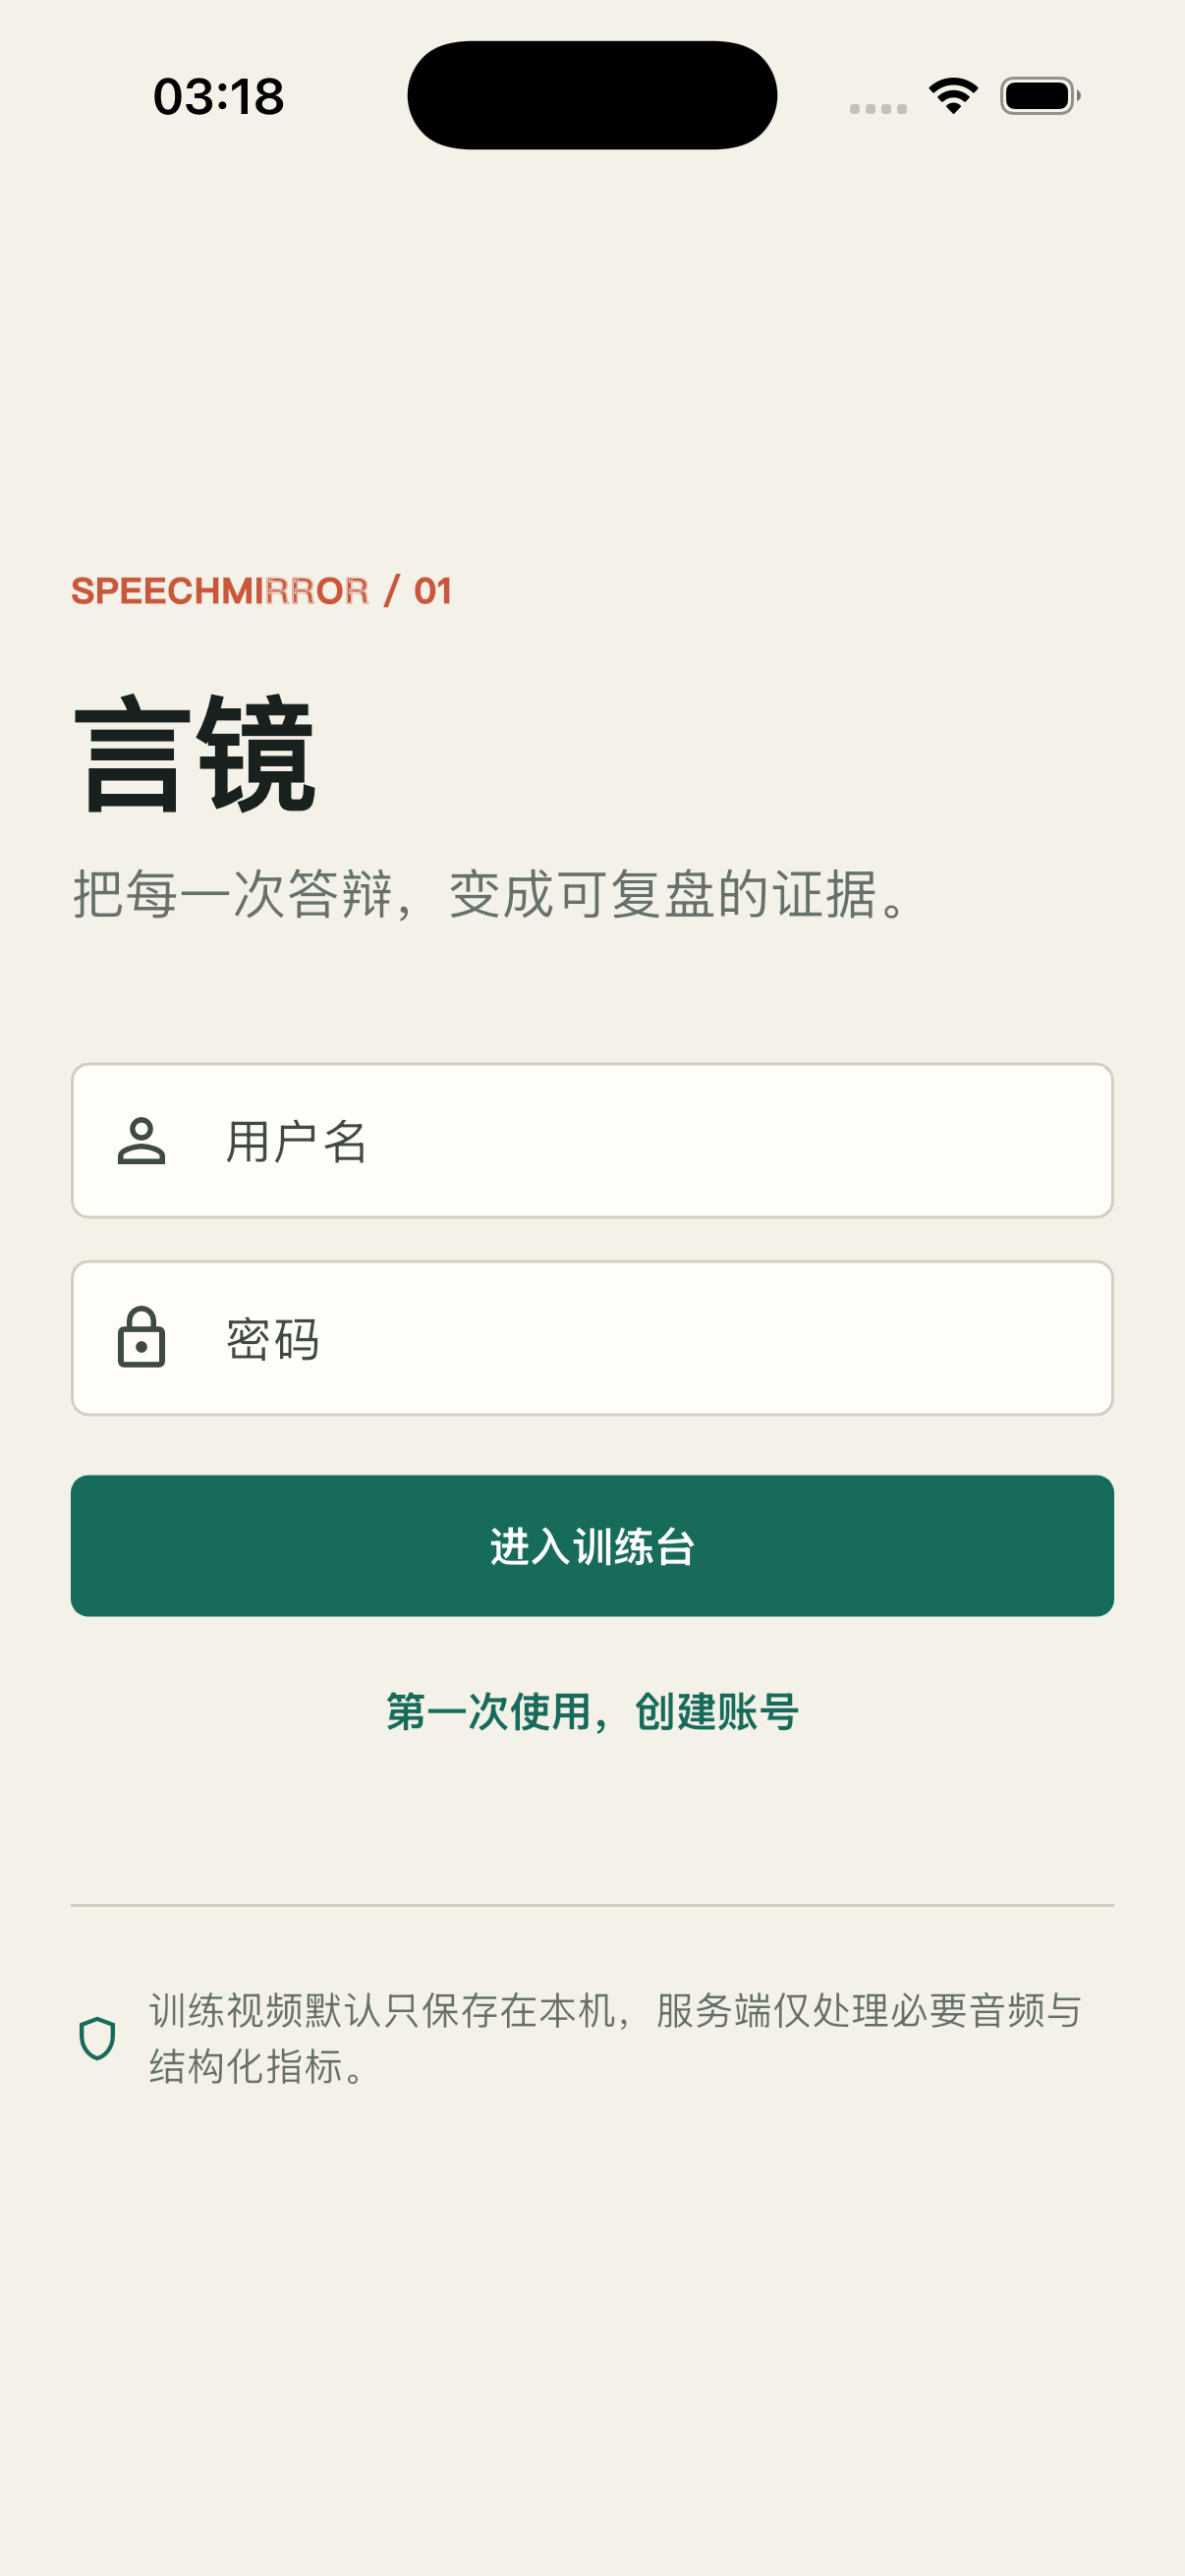
\includegraphics[width=\linewidth]{figures/login_screen.png}
  \caption{iOS Simulator}
\end{subfigure}
\hfill
\begin{subfigure}[t]{0.42\textwidth}
  \centering
  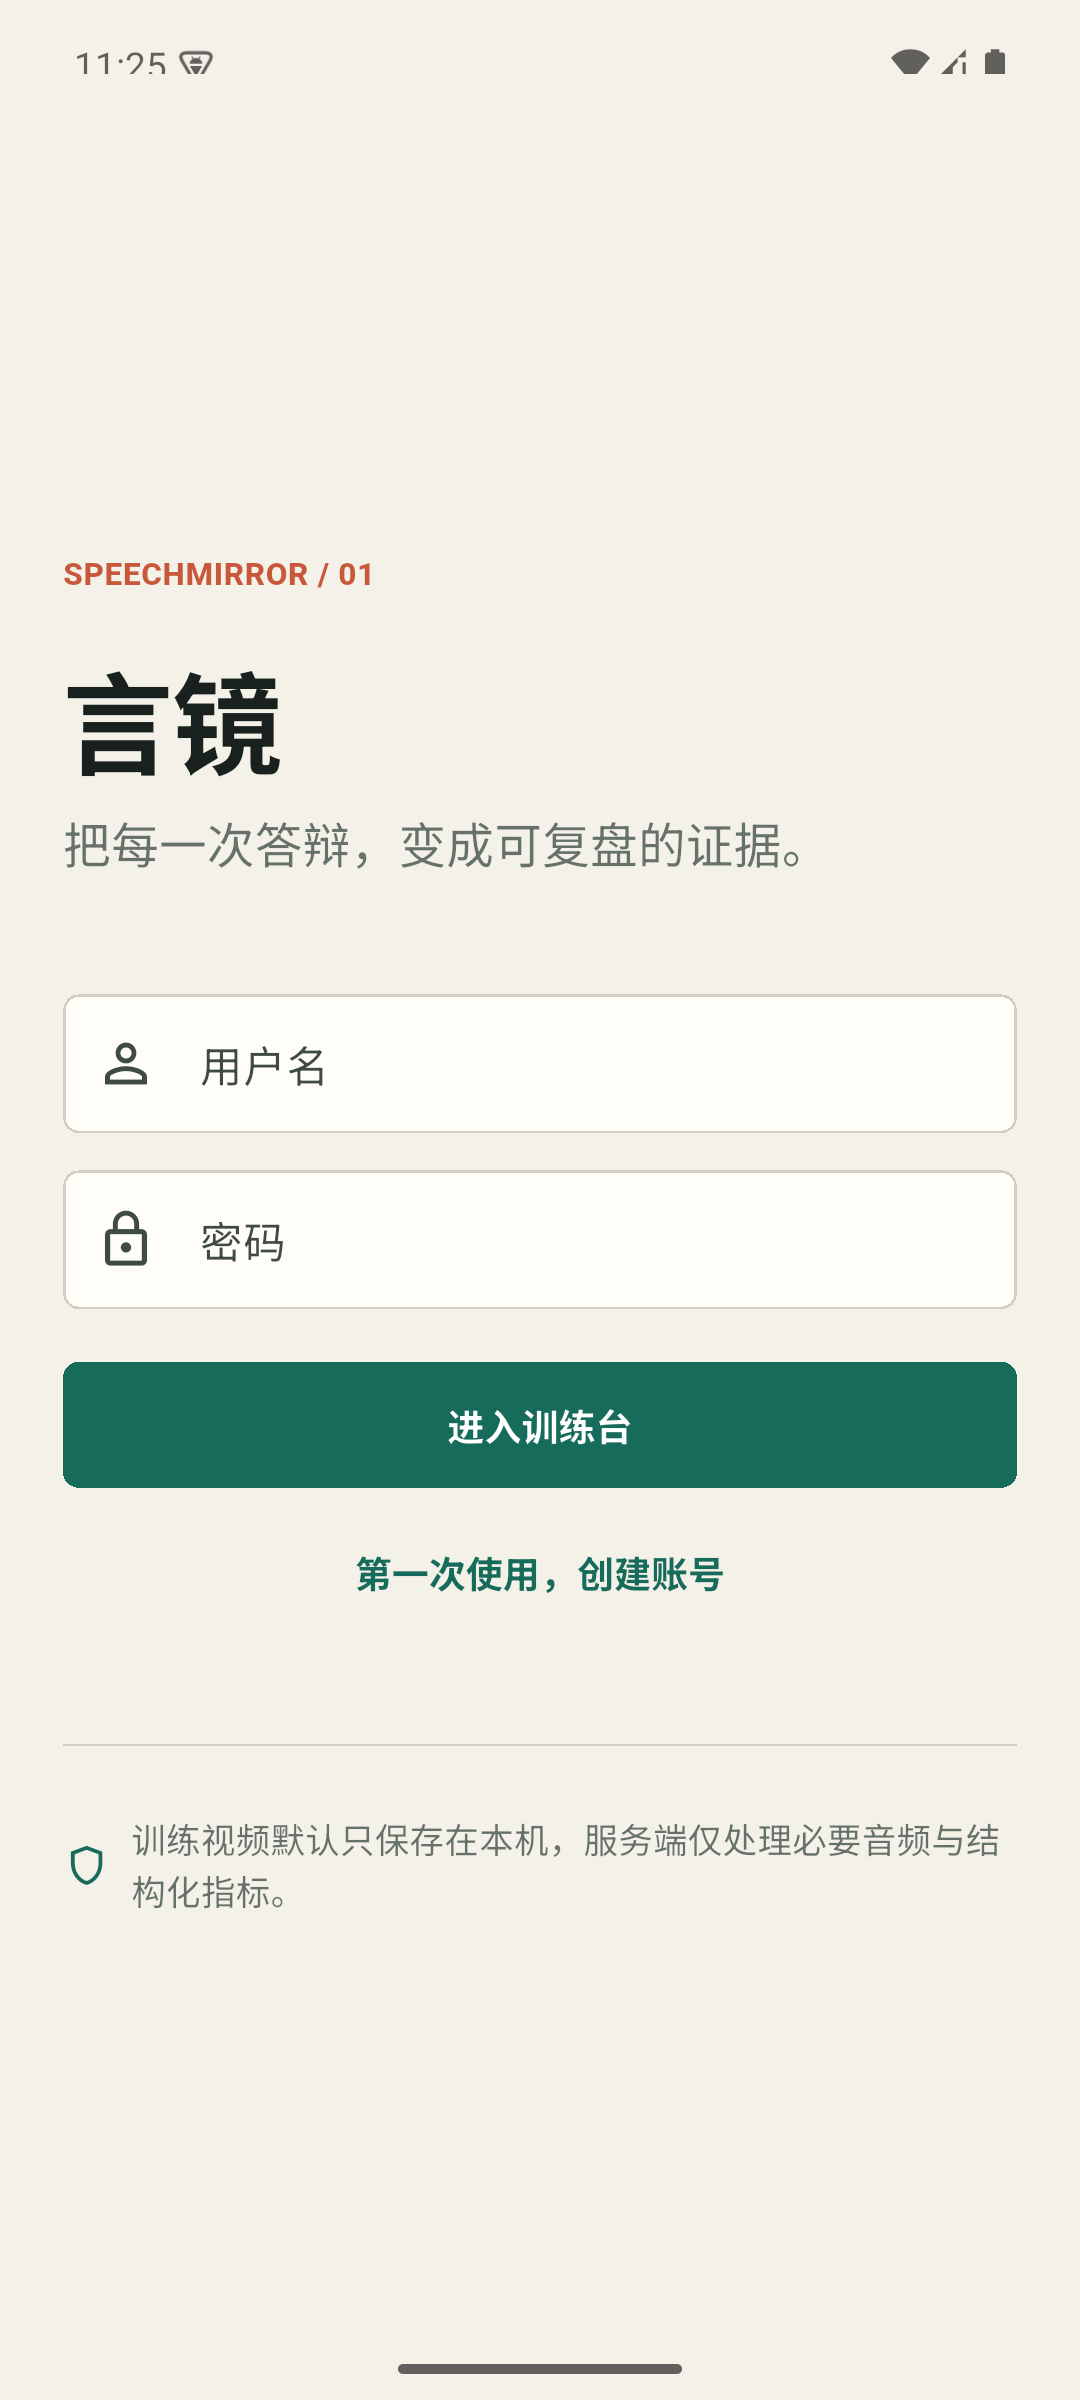
\includegraphics[width=\linewidth]{figures/android_login_screen.png}
  \caption{Android Emulator}
\end{subfigure}
\caption{Flutter登录页在iOS与Android中的实际运行截图}
\end{figure}

\begin{figure}[H]
\centering
\begin{subfigure}[t]{0.36\textwidth}
  \centering
  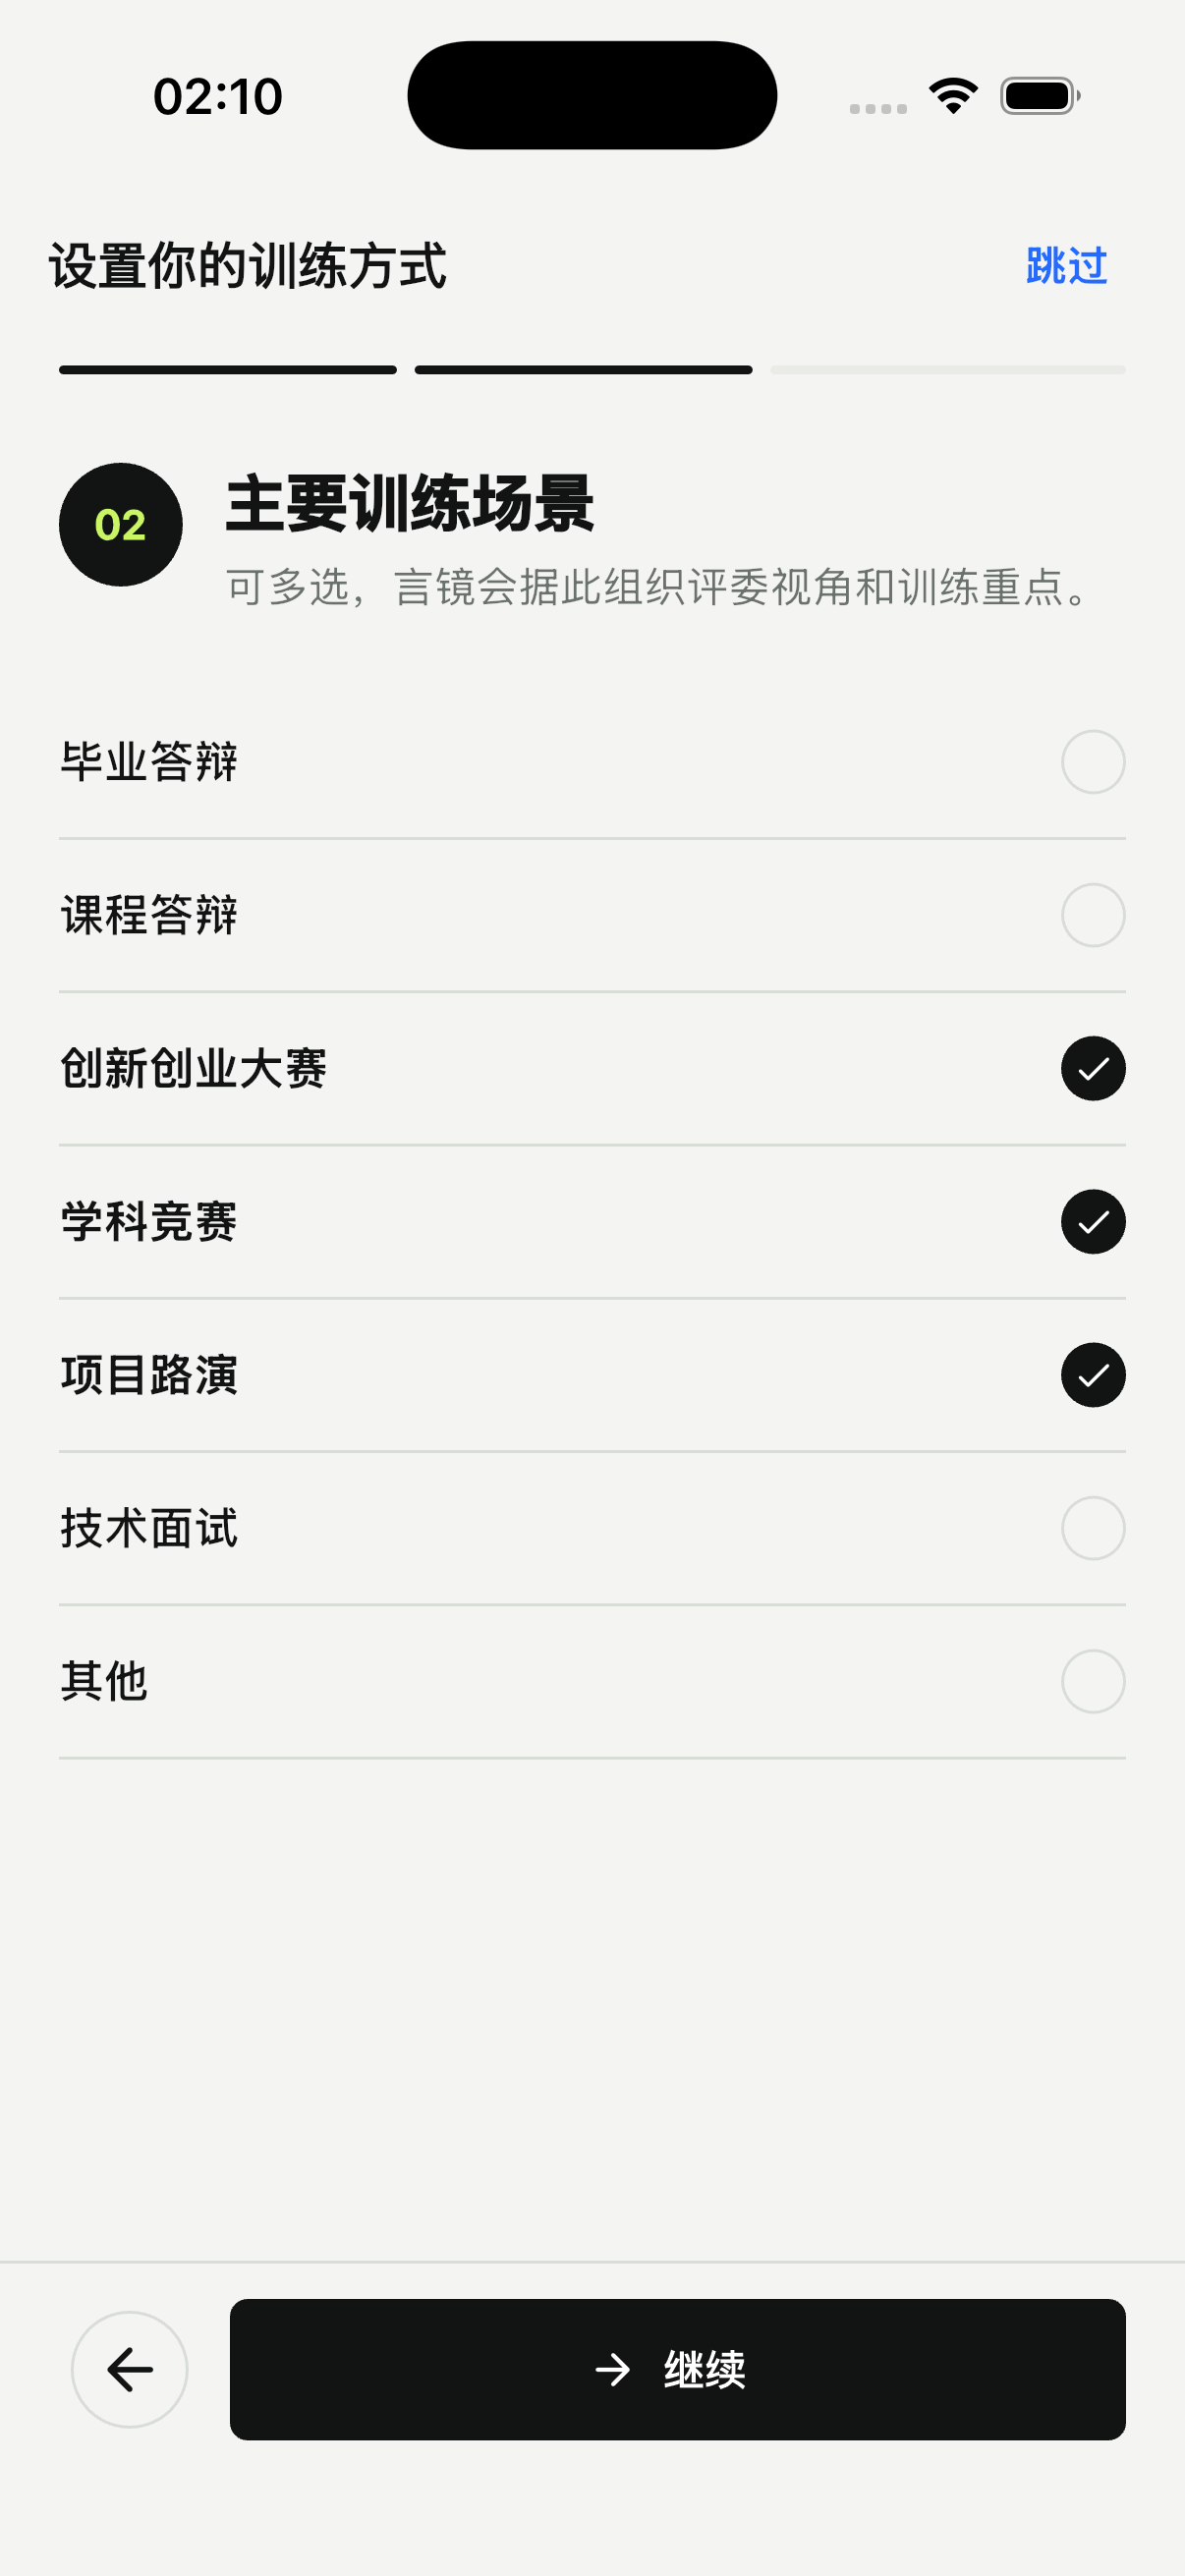
\includegraphics[width=\linewidth]{figures/onboarding_scenarios.png}
  \caption{训练场景多选}
\end{subfigure}
\hfill
\begin{subfigure}[t]{0.36\textwidth}
  \centering
  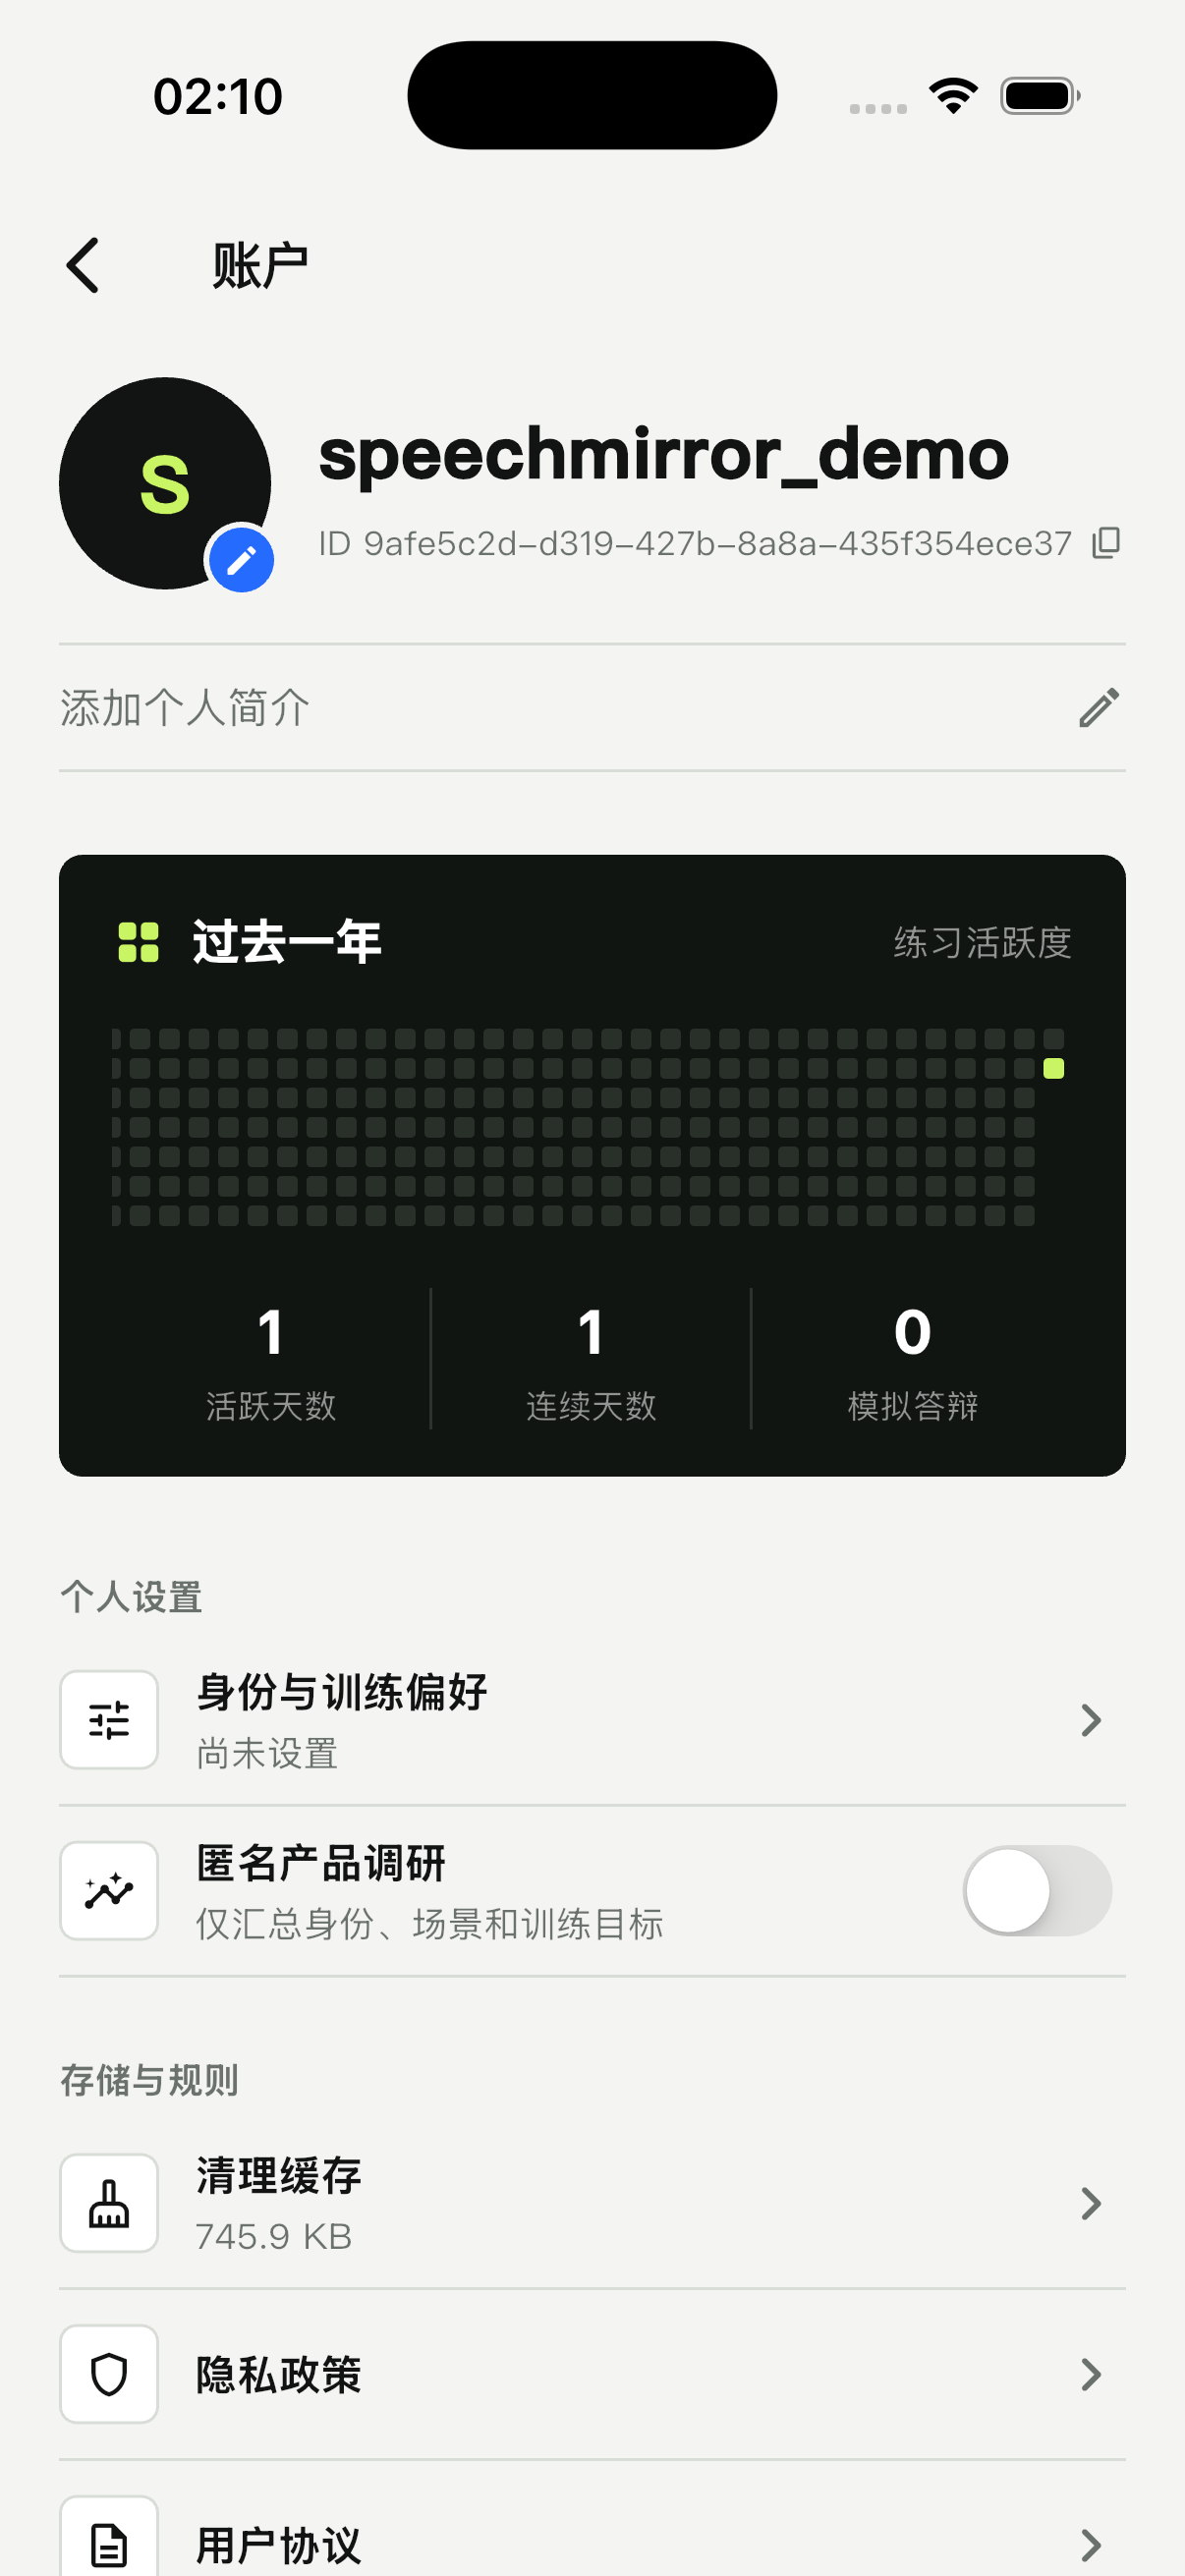
\includegraphics[width=\linewidth]{figures/user_center.png}
  \caption{用户中心与活跃点阵}
\end{subfigure}
\caption{iOS模拟器中的首次引导与用户中心实际截图}
\end{figure}

\chapter{HarmonyOS 6原生适配与创新}
\section{原生工程}
HarmonyOS工程包含AppScope、entry HAP、Stage EntryAbility、ArkUI页面、NetworkKit请求层和N-API模块。登录、项目、材料状态、训练、报告与评委页面沿用统一信息架构，但控件和生命周期由ArkUI原生实现，不嵌入Flutter或网页。

\section{系统能力协同}
训练页已经建立XComponent surface边界，并通过Vibrator在达到目标时长时提供一次低干扰提醒。页面只显示当前时长、目标时长和录制状态，不用连续弹窗打断表达。媒体管线未产生有效录制结果时，界面明确提示且不上传文件、不生成分析数据，从交互层保持失败显式原则。

\section{隐私友好的端云协同}
HarmonyOS工程通过N-API加载共享C++库并读取ABI版本，用同一二进制边界约束后续结构化指标。服务端没有视频上传路由，原生客户端也不把XComponent画面提交到网络层，因此视频本地化不是单纯依赖隐私政策文本，而是由接口能力共同限制。视觉维度没有结构化采样时保持空值，不用随机指标补齐报告。

\section{适配价值与边界}
HarmonyOS版本以原生页面访问统一的项目、材料、会话和报告接口，并与iOS、Android共用端侧指标口径。其创新点不是将网页封装为应用，而是把ArkUI原生交互、N-API共享ABI与服务端材料检索组成统一的端云协同路径。该设计面向我国自主移动操作系统生态，降低单一平台依赖，不对操作系统或第三方技术作产权归属表述。

\section{国产基础软件与AI生态协同}
项目的技术立场是让核心能力建立在公开契约和可替换边界上，而不是简单堆叠国产技术名词。HarmonyOS 6负责原生终端交互、媒体权限、本地数据与端侧隐私边界；DeepSeek负责材料约束下的问题生成与语言反馈；Rust后端负责鉴权、检索、证据校验和数据生命周期。三者通过OpenAPI、Provider接口和结构化指标连接，任何单一模型或移动平台的变化都不要求重写全部业务逻辑。

这种组合形成两个层面的工程价值。第一，国产移动操作系统获得独立原生工程和统一业务入口，核心业务契约不再只依附iOS和Android生态；第二，国产开放模型通过标准接口进入应用架构，并保留自主部署或替换模型的可能。创新点因此落在“国产终端原生适配、国产模型开放接口、端云隐私协同、材料证据约束”四项可检查的系统机制上，而不是将模型生成结果包装成无法解释的总分。

\chapter{隐私、安全与伦理边界}
\section{数据最小化}
系统收集实现功能所需的最小数据。账号不要求真实姓名和手机号；音频只为ASR临时传输；视觉上传的是数值指标；报告保留转写和材料引用以供复盘。个人信息处理应遵循目的明确、最小必要和公开透明原则\cite{pipl}。

身份、训练场景和提升目标用于调整产品体验，与匿名产品调研用途分开。research\_consent默认关闭，用户可以跳过引导或在用户中心随时关闭。即使用户打开该开关，也只允许汇总身份、场景和训练目标，不允许把论文材料、录音、视频、答辩回答或报告用于这一调研目的。该边界同时写入引导页说明、用户中心副标题和应用内隐私政策。

\section{传输与存储}
密码只保存Argon2id摘要，刷新令牌只保存哈希。SQLite、材料与日志使用持久卷，备份文件应加密并限制访问。日志不记录Authorization头、音频正文、完整转写或AI密钥。生产环境必须替换开发JWT密钥并启用HTTPS；当前测试地址用于受控调试，不被描述为正式生产域名。

头像上传属于独立接口，最大2~MiB，只允许通过文件头识别出的PNG或JPEG。客户端缓存清理仅删除系统临时目录和内存图片缓存，不递归清理应用文档目录，因此断网后保留的待提交训练媒体不会被“清理缓存”误删。用户删除头像、项目或退出登录分别具有清楚边界，不把退出登录等同于删除业务数据。

\section{提示注入与材料污染}
用户材料可能包含“忽略此前要求”等指令性文本。材料在系统中是待评价的数据而非系统指令，提示模板要明确这一层级。引用必须检查chunk\_id，输出展示引文而不是只展示模型总结。对上传文件还应限制尺寸、类型、转换超时和解析进程权限。

\section{评价伦理}
系统只评价可观察行为和材料覆盖，不评价情绪、人格、可信度、心理疾病或就业能力。分数不是排名，也不是教师成绩。模型置信不应被包装为科学测量。用户可以删除项目及其服务端派生数据，本地视频由用户自行管理。

\section{应用内告知与用户控制}
客户端内置隐私政策和用户协议页面，说明账号、材料、训练、AI供应商、缓存、删除和研究同意等处理规则。用户中心提供复制用户ID、编辑简介和偏好、移除头像、清理缓存、撤回匿名调研同意及退出登录入口。研究同意不是使用应用的必要条件，关闭后不影响项目、训练、问答和报告功能。这种设计把告知、选择和撤回放入实际交互，而不是仅在论文中作原则性声明。

\chapter{部署与运维}
\section{容器部署}
后端Docker镜像采用Rust构建阶段和Debian运行阶段。运行镜像安装LibreOffice、Poppler、Noto CJK字体和CA证书，以非root用户启动。Compose只包含API与Caddy，不引入Redis；SQLite、材料和Caddy证书使用命名卷。

\section{配置管理}
环境变量包括\path{BIND_ADDR}、\path{DATABASE_URL}、\path{STORAGE_DIR}、\path{JWT_SECRET}、\path{CORS_ALLOWED_ORIGINS}，以及LLM、Embedding、ASR、OCR各自的服务地址、密钥和模型名。\texttt{.env}被Git忽略，仓库只提供\texttt{.env.example}。浏览器跨域访问默认关闭，只能按明确的HTTPS来源白名单开启；移动端通过编译参数设置API基址，生产环境只使用HTTPS。

\section{日志与健康检查}
Tracing输出结构化请求日志，健康接口返回\path{status}、\path{ai_configured}和四项Provider配置状态。健康检查不调用付费模型，也不泄露模型密钥。请求日志不记录Authorization头和媒体正文，以日志轮换限制本地保留量。

\section{备份恢复}
备份SQLite时应使用在线备份API或在短暂停写窗口复制数据库及WAL相关文件，不能只复制主文件。材料卷与数据库快照需要同一恢复点。恢复演练应检查用户登录、材料状态、报告读取和新任务领取。

\chapter{软件测试与结果}
\section{测试策略}
测试分为单元、接口集成、组件、构建、真机回归和非功能测试。Rust单元与接口测试覆盖分块、口头禅与停顿统计、材料引文强校验、问题序号清洗、问题去重、未知回答换题、评分上限、注册、JWT轮换、项目管理、用户画像、头像约束、活跃日期和多选场景持久化。Flutter测试覆盖报告与画像模型解析、首次引导跳过、同时保存两个训练场景、缓存清理不删除应用文档中的待提交媒体、项目管理和答辩追问状态。C++测试覆盖ABI和未加载模型的失败路径。构建验证用于证明产物可生成，但不代替设备运行。

\section{已执行结果}
\begin{longtable}{p{3.6cm}p{5.0cm}p{5.9cm}}
\caption{截至2026年9月29日的真实执行结果}\\
\toprule 对象 & 命令 & 结果 \\
\midrule
\endfirsthead
\toprule 对象 & 命令 & 结果 \\
\midrule
\endhead
Rust API & \texttt{cargo test} & 38项测试通过，0失败 \\
Rust API & \texttt{cargo clippy --all-targets --all-features -- -D warnings} & 通过，0项警告 \\
本地HTTP & \texttt{curl}真实请求 & 健康、注册、项目创建、Markdown上传及ready状态通过 \\
任务队列 & 可控Provider集成测试 & 回答ASR、训练ASR和报告任务独立运行，结果字段相互隔离 \\
Flutter & \texttt{flutter analyze} & 0项问题 \\
Flutter & \texttt{flutter test} & 27项测试通过，0失败 \\
Android & \texttt{flutter build apk --debug} & 成功生成调试APK，约163 MB \\
iOS模拟器 & 可视化回归 & 登录、三步引导、多选场景、用户中心和活跃点阵显示通过 \\
iOS真机 & Profile构建与安装 & 生成33.8 MB Runner.app，并成功安装到iPhone 15 Pro \\
公网VPS & 迁移与真实API请求 & 健康状态为ok，LLM、Embedding、ASR、OCR均为已配置；多场景画像读写通过 \\
C++核心 & \texttt{cmake; ctest} & 1项ABI契约测试通过 \\
OpenAPI & Ruby YAML解析 & 3.1.0文档可解析，共24条路径 \\
\bottomrule
\end{longtable}

\section{结果判定原则}
测试记录包含日期、提交版本、运行环境、输入材料和命令输出。自动化检查以进程退出码和断言结果为准，构建检查只证明目标产物可生成，不代替业务结果评估。截图与日志在进入论文前移除令牌、密钥和个人材料。

\chapter{系统使用说明}
\section{部署服务端}
在VPS安装Docker与Compose，复制环境变量样例，生成至少32字节随机JWT密钥并填写AI供应商凭据。无域名调试阶段可仅发布受控HTTP端口；配置域名后由Caddy反向代理API并申请HTTPS证书。运行\texttt{docker compose up -d --build}，确认健康接口为ok且LLM、Embedding、ASR和OCR配置状态符合当前功能。定期备份数据卷。

\section{安装移动端}
Android通过APK进行调试安装，安装包使用SHA-256校验。iOS通过Xcode和开发者签名安装到测试设备，不包含App Store发布流程。HarmonyOS使用DevEco Studio配置签名并安装HAP，运行记录同时保存SDK和设备版本。

\section{完成首次设置}
注册登录后可以直接跳过首次设置，也可以依次选择身份、一个或多个训练场景以及一个或多个提升目标。选择“其他”时填写补充文本。匿名产品调研默认关闭，不影响后续功能。进入项目列表后点击用户中心，可以修改头像、简介和训练偏好，查看365天活跃点阵，清理临时缓存，并阅读隐私政策与用户协议。

\section{创建项目与材料}
登录后新建项目，设置名称、说明和目标时长。上传材料后等待状态变为“已完成解析”。扫描文件应打开提取文本检查错字；若关键信息错误，先纠正再训练。材料状态失败时查看错误，不应继续生成问题。

\section{完成一次训练}
将手机置于稳定位置，使头肩位于画面中央。进入模拟答辩后先面对镜头完整介绍项目；界面使用正计时，达到目标时间仅振动一次而不强制结束。介绍完成后点击按钮进入答辩，继续面对镜头听取评委提问并逐题回答。AI提问、识别和思考期间计时暂停，只累计答辩者的陈述与回答时间。网络失败时系统最多自动重试五次，达到上限后可手动重试，本地媒体继续保留。

\section{阅读报告与问答}
答辩结束后先看九项综合评分与最大问题，再查看时间、语速、长停顿和口头禅等确定性指标。内容与问答评价应同时显示材料引文、已覆盖要点、缺失要点和改进建议；详细推理默认折叠，需要复核时再展开。建议优先准备报告列出的具体问题，并在下一次训练中比较同一项目的变化。

\chapter{结论}
本文给出了SpeechMirror从需求边界、数据模型、接口、材料知识库、AI评委、端侧指标到多端客户端和容器化部署的工程实现。系统把真实答辩拆分为完整陈述、材料阅读、逐题问答、动态追问和结束后评分五个连续阶段，并用统一会话保存转写、问题、回答、证据和报告。问题生成同时使用项目材料、现场陈述与历史问答，通过序号清洗、单问题约束、材料校验和相似度去重避免模板化提问；回答评价又通过确定性分数上限抑制跑题、胡编和无材料依据造成的虚高分。

Flutter客户端实现全屏陈述与答辩、正计时、五次自动重试、自然中文音色、默认折叠推理和稳定返回项目流程。新增用户中心与三步可跳过引导，支持头像、简介、多选训练场景、多选目标、365天活跃点阵、缓存清理及应用内隐私政策和用户协议。研究同意默认关闭且范围明确，个人偏好与认证数据分表存储，多场景迁移兼容旧客户端。

DeepSeek语言模型Provider与向量、ASR、OCR配置彼此隔离，既利用国产开放模型生态，又避免把供应商能力范围写得过宽。Rust接口、SQLite持久化队列、Flutter工作流、C++ ABI以及24条OpenAPI路径共同构成可复现的实现基线。自动化验证达到Rust 38项和Flutter 27项测试全部通过，iOS Profile产物已经安装到iPhone 15 Pro，公网VPS完成画像多场景接口与迁移验证。

HarmonyOS 6客户端以ArkTS、ArkUI、Stage模型和N-API组织原生工程，与Flutter客户端共用业务契约和端侧指标定义。这一实现面向我国自主移动操作系统生态，将原生交互、端侧数据最小化与服务端可解释分析结合。国产开放模型与国产移动操作系统分别承担云侧语言理解和端侧原生体验，通过公开接口形成可替换、可审计的协同关系，体现了多端迁移、端云协同和隐私边界一致性的设计价值。

\printbibliography[heading=bibintoc,title={参考文献}]
\appendix
\chapter{接口摘要}
\begin{longtable}{>{\raggedright\arraybackslash}p{4.5cm}>{\raggedright\arraybackslash}p{2.7cm}p{6.8cm}}
\toprule 路径 & 方法 & 用途 \\
\midrule
\endfirsthead
\toprule 路径 & 方法 & 用途 \\
\midrule
\endhead
/auth/register & POST & 注册并签发令牌 \\
/auth/login & POST & 登录并签发令牌 \\
/auth/refresh & POST & 轮换刷新令牌 \\
/auth/logout & POST & 撤销当前刷新令牌 \\
/me & GET/PUT & 读取或更新简介、身份、多选场景、目标和调研同意 \\
/me/avatar & GET/\allowbreak POST/\allowbreak DELETE & 读取、上传或删除PNG/JPEG头像，最大2~MiB \\
/me/activity & GET/POST & 读取365天活跃记录或记录当日使用 \\
/projects & GET/POST & 项目列表与创建 \\
/projects/\{id\} & GET/\allowbreak PUT/\allowbreak DELETE & 项目读取、更新和彻底删除 \\
/projects/\{id\}/\allowbreak documents & GET/\allowbreak POST & 材料列表与上传 \\
/documents/\{id\} & GET & 读取材料元数据、状态和提取文本 \\
/documents/\{id\}/\allowbreak text & PUT & 纠正并重新索引文本 \\
/projects/\{id\}/\allowbreak sessions & GET/\allowbreak POST & 训练历史与创建 \\
/sessions/\{id\} & GET & 读取训练会话和处理状态 \\
/sessions/\{id\}/\allowbreak metrics & POST & 上传端侧派生指标 \\
/sessions/\{id\}/\allowbreak audio & POST & 临时音频ASR \\
/sessions/\{id\}/\allowbreak answer-audio & POST & 回答音频临时转写，不覆盖训练转写 \\
/sessions/\{id\}/\allowbreak complete & POST & 完成训练 \\
/sessions/\{id\}/\allowbreak analyze & POST & 生成报告 \\
/sessions/\{id\}/\allowbreak report & GET & 读取报告 \\
/projects/\{id\}/\allowbreak questions & GET/\allowbreak POST & 问题列表与生成 \\
/questions/\{id\}/\allowbreak answers & POST & 提交回答并评价 \\
/projects/\{id\}/\allowbreak trends & GET & 历史趋势 \\
\bottomrule
\end{longtable}

完整机器可读契约见仓库\texttt{openapi/openapi.yaml}。

\chapter{数据约束摘要}
\begin{longtable}{>{\raggedright\arraybackslash}p{4.5cm}>{\raggedright\arraybackslash}p{4.8cm}p{5.4cm}}
\toprule 对象 & 关联与索引 & 一致性规则 \\
\midrule
\endfirsthead
\toprule 对象 & 关联与索引 & 一致性规则 \\
\midrule
\endhead
users & username唯一索引 & 只保存Argon2id密码摘要 \\
\path{user_profiles} & \path{user_id}唯一外键 & 调研同意默认false；多场景数组为规范字段，旧单场景字段用于兼容 \\
\path{user_activity_days} & \path{(user_id, activity_date)}联合主键 & 当地日期只允许在UTC日期前后一日内；分别累计使用与练习次数 \\
\path{refresh_tokens} & \path{user_id}外键 & 只保存SHA-256摘要，刷新时原子撤销 \\
projects & \path{user_id}外键 & 所有读写均按当前用户过滤 \\
documents & \path{project_id}外键 & 状态在processing、ready和failed之间迁移 \\
\path{document_chunks} & \path{document_id}与\path{project_id} & 引文必须逐字属于当前项目片段 \\
\path{analysis_jobs} & \path{resource_id}索引 & 任务状态及\path{result_json}持久化 \\
\path{rehearsal_sessions} & \path{project_id}与\path{user_id} & 会话、问题与回答项目必须一致 \\
reports & \path{session_id}唯一关联 & 未采集维度以null表达 \\
\path{jury_questions} & \path{project_id}与\path{session_id} & 问题证据只能引用当前项目材料 \\
\path{jury_answers} & \path{question_id}与\path{session_id} & 回答评价不覆盖训练转写 \\
\bottomrule
\end{longtable}

\chapter{可复现验证命令}
\begin{lstlisting}[language=bash,caption={代码与论文验证命令}]
cd services/api
cargo fmt --check
cargo test
cargo clippy --all-targets --all-features -- -D warnings

cd apps/flutter_mobile
flutter analyze
flutter test
flutter build apk --debug
flutter build ios --profile --no-codesign

cd native/edge_vision
cmake -S . -B build
cmake --build build
ctest --test-dir build --output-on-failure

cd docs/paper
make render
\end{lstlisting}

\chapter{答辩决策与评分约束摘要}
\begin{longtable}{>{\raggedright\arraybackslash}p{4.0cm}>{\raggedright\arraybackslash}p{4.8cm}p{5.9cm}}
\toprule 规则对象 & 实现约束 & 用户可见结果 \\
\midrule
\endfirsthead
\toprule 规则对象 & 实现约束 & 用户可见结果 \\
\midrule
\endhead
项目介绍 & 用户明确结束后才进入评委阶段 & 介绍期间不被提前提问 \\
长停顿 & 检测到有效语音后才累计静音区间 & 开头准备时间不记为长停顿 \\
主问题 & 一次只生成并播报一个核心问题 & 不出现多题连问和列表编号 \\
追问 & 只核查一个关键漏洞，最多两层 & 模糊回答被追问，明确不会则换题 \\
结束条件 & 至少3道主问题；最多10道主问题或14轮回答 & 题数随覆盖程度变化，不设置倒计时 \\
计时 & 模型、识别和播报阶段暂停 & 显示答辩者累计表达时间 \\
自动恢复 & 外部请求最多重试5次 & 显示当前次数，之后提供手动重试 \\
评分 & 原始模型分受材料与覆盖规则限制 & 跑题、胡编和无依据回答不能获得高分 \\
详细评价 & 默认折叠，保留手动展开 & 首屏突出证据、缺失点和改进建议 \\
\bottomrule
\end{longtable}

\chapter{用户画像与隐私字段摘要}
\begin{longtable}{>{\raggedright\arraybackslash}p{4.0cm}>{\raggedright\arraybackslash}p{4.7cm}p{6.0cm}}
\toprule 字段或功能 & 数据形式 & 边界 \\
\midrule
\endfirsthead
\toprule 字段或功能 & 数据形式 & 边界 \\
\midrule
\endhead
identity & 单选枚举与可选其他文本 & 可跳过，可在用户中心修改 \\
scenarios & 去重字符串数组，最多7项 & 支持毕业答辩、课程答辩、竞赛、路演、面试和其他多选 \\
purposes & 去重字符串数组与可选其他文本 & 用于记录多个训练目标 \\
research\_consent & 布尔值，默认false & 只允许汇总身份、场景与目标，不包含训练内容 \\
avatar & PNG或JPEG二进制，最大2~MiB & 读取、替换与删除均要求本人令牌 \\
activity & 365个每日计数 & 展示活跃度，不形成用户排名 \\
cache & 系统临时目录与图片缓存 & 不删除应用文档目录中的待提交训练媒体 \\
\bottomrule
\end{longtable}

\chapter{关键配置说明}
\begin{longtable}{>{\raggedright\arraybackslash}p{5.7cm}p{8.7cm}}
\toprule 环境变量 & 用途 \\
\midrule
\endfirsthead
\toprule 环境变量 & 用途 \\
\midrule
\endhead
\path{BIND_ADDR} & Axum监听地址与端口 \\
\path{DATABASE_URL} & SQLite数据库连接串 \\
\path{STORAGE_DIR} & 材料、临时音频与中间文件目录 \\
\path{JWT_SECRET} & JWT签名密钥，最少32个字符 \\
\path{CORS_ALLOWED_ORIGINS} & 允许的浏览器HTTPS来源白名单 \\
\path{LLM_BASE_URL} / \path{LLM_API_KEY} / \path{LLM_MODEL} & DeepSeek语言模型地址、凭据与模型名 \\
\path{EMBEDDING_BASE_URL} / \path{EMBEDDING_API_KEY} / \path{EMBEDDING_MODEL} & 材料片段与查询向量化服务配置 \\
\path{ASR_BASE_URL} / \path{ASR_API_KEY} / \path{ASR_MODEL} & 训练与评委回答语音识别服务配置 \\
\path{OCR_BASE_URL} / \path{OCR_API_KEY} / \path{OCR_MODEL} & 扫描页面与图片文字识别服务配置 \\
\bottomrule
\end{longtable}

密钥只通过服务端环境变量注入，不写入论文、截图、Git仓库或客户端。模型变更后重新执行材料检索、问答和报告回归测试。

\end{document}
